\begin{pastexam}[label={px:ncku-108-ee-ds-08}]{成大電機所 108 學年度 問答題第 7 題}
（問答）

An AVL (Adelson-Velsky and Landis) tree is a self-balancing binary search tree. Please draw the
resulting AVL tree after inserting the following numbers under the root with no subtree. Please show
your answer step by step. (10 points)

\quad \{add(8); add(9); add(10); add(2); add(1); add(5); add(3); add(6); add(4); add(7);\}
\end{pastexam}

\begin{pastsoln}
題目的「under the root with no subtree」指從空樹開始插入。 每次照 BST 插入（資結書第~9.2~節），再從新節點
往上找第一個平衡因子（左子樹高減右子樹高）變成 $\pm 2$ 的節點，依新節點落在它的哪一邊做 LL、RR、LR、RL
旋轉（資結書第~10.2.3~節）。 一次插入最多只要在這個節點做一次（單或雙）旋轉。

下面每一步畫出做完旋轉之後的樹。

\begin{center}
\begin{tikzpicture}[every node/.style={circle, draw, minimum size=6mm, inner sep=0pt, font=\small},
    level distance=8.5mm, level 1/.style={sibling distance=13mm}, level 2/.style={sibling distance=7mm},
    lab/.style={draw=none, rectangle, font=\footnotesize, align=center}]
\node at (0,0) {8};
\node[lab] at (0,-2.4) {(1) add 8};
\begin{scope}[xshift=2.6cm]
\node {8} child[missing] child {node {9}};
\node[lab] at (0,-2.4) {(2) add 9};
\end{scope}
\begin{scope}[xshift=5.6cm]
\node {9} child {node {8}} child {node {10}};
\node[lab] at (0,-2.4) {(3) add 10\\ 8 失衡，RR};
\end{scope}
\begin{scope}[xshift=9.0cm]
\node {9} child {node {8} child {node {2}} child[missing]} child {node {10}};
\node[lab] at (0,-2.4) {(4) add 2};
\end{scope}
\begin{scope}[xshift=12.4cm]
\node {9} child {node {2} child {node {1}} child {node {8}}} child {node {10}};
\node[lab] at (0,-2.4) {(5) add 1\\ 8 失衡，LL};
\end{scope}
\end{tikzpicture}
\end{center}

\begin{center}
\begin{tikzpicture}[every node/.style={circle, draw, minimum size=6mm, inner sep=0pt, font=\small},
    level distance=8.5mm, level 1/.style={sibling distance=15mm}, level 2/.style={sibling distance=8.5mm},
    level 3/.style={sibling distance=7mm},
    lab/.style={draw=none, rectangle, font=\footnotesize, align=center}]
\node {8} child {node {2} child {node {1}} child {node {5}}} child {node {9} child[missing] child {node {10}}};
\node[lab] at (0,-3.55) {(6) add 5\\ 9 失衡，LR};
\begin{scope}[xshift=4.25cm]
\node {8} child {node {2} child {node {1}} child {node {5} child {node {3}} child[missing]}}
  child {node {9} child[missing] child {node {10}}};
\node[lab] at (0,-3.55) {(7) add 3};
\end{scope}
\begin{scope}[xshift=8.5cm]
\node {8} child {node {2} child {node {1}} child {node {5} child {node {3}} child {node {6}}}}
  child {node {9} child[missing] child {node {10}}};
\node[lab] at (0,-3.55) {(8) add 6};
\end{scope}
\begin{scope}[xshift=12.75cm]
\node {8} child {node {3} child {node {2} child {node {1}} child[missing]} child {node {5} child {node {4}} child {node {6}}}}
  child {node {9} child[missing] child {node {10}}};
\node[lab] at (0,-3.55) {(9) add 4\\ 2 失衡，RL};
\end{scope}
\end{tikzpicture}
\end{center}

各步說明：
\begin{enumerate}
\item add 8：空樹，$8$ 是根。
\item add 9：$9 > 8$，接在 $8$ 右邊。 $8$ 的平衡因子 $-1$。
\item add 10：接在 $9$ 右邊。 $8$ 的平衡因子 $-2$，新節點在 $8$ 的右子節點的右邊：\textbf{RR}，對 $8$ 左旋，
$9$ 成為根。
\item add 2：$2 < 9$、$2 < 8$，接在 $8$ 左邊。 $8$ 是 $+1$，$9$ 是 $+1$，平衡。
\item add 1：接在 $2$ 左邊。 往上第一個失衡的是 $8$（$+2$），新節點在它左子節點的左邊：\textbf{LL}，對 $8$ 右旋，
$2$ 取代 $8$ 的位置，$8$ 成為 $2$ 的右子節點。
\item add 5：$5 < 9$、$5 > 2$、$5 < 8$，接在 $8$ 左邊。 $8$ 是 $+1$、$2$ 是 $-1$，$9$ 的左子樹高 $3$、右子樹高 $1$，
$+2$ 失衡；新節點在 $9$ 的左子節點 $2$ 的右邊：\textbf{LR}。 先對 $2$ 左旋、再對 $9$ 右旋，$8$ 成為根，左子節點
$2$（子節點 $1$、$5$），右子節點 $9$（右子節點 $10$）。
\item add 3：$3 < 8$、$3 > 2$、$3 < 5$，接在 $5$ 左邊。 $5$ 是 $+1$，$2$ 是 $-1$，$8$ 是 $+1$，平衡。
\item add 6：接在 $5$ 右邊。 $5$ 是 $0$，$2$ 是 $-1$，$8$ 是 $+1$，平衡。
\item add 4：$4 < 8$、$4 > 2$、$4 < 5$、$4 > 3$，接在 $3$ 右邊。 $3$ 是 $-1$，$5$ 是 $+1$，$2$ 的左子樹高 $1$、右子樹
高 $3$，$-2$ 失衡；新節點在 $2$ 的右子節點 $5$ 的左邊：\textbf{RL}。 先對 $5$ 右旋、再對 $2$ 左旋，$3$ 取代 $2$
的位置：$3$ 的左子節點 $2$（$2$ 的左子節點 $1$），右子節點 $5$（子節點 $4$、$6$）。 這棵子樹高度回到 $3$，
$8$ 是 $+1$，不必再往上處理。
\item add 7：$7 < 8$、$7 > 3$、$7 > 5$、$7 > 6$，接在 $6$ 右邊。 $6$ 是 $-1$，$5$ 是 $-1$，$3$ 是 $-1$，$8$ 的左子樹高
$4$、右子樹高 $2$，$+2$ 失衡；新節點在 $8$ 的左子節點 $3$ 的右邊：\textbf{LR}。 先對 $3$ 左旋（$5$ 上來，$5$
原本的左子樹 $4$ 變成 $3$ 的右子樹），再對 $8$ 右旋（$5$ 成為根，$5$ 原本的右子樹 $6$ 變成 $8$ 的左子樹）。
\end{enumerate}

\textbf{最後的 AVL 樹}：
\begin{center}
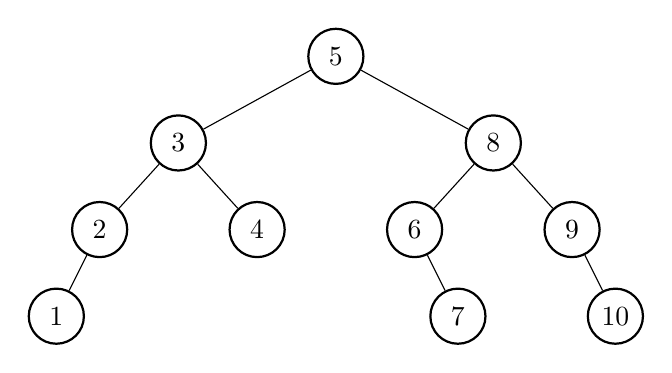
\begin{tikzpicture}[every node/.style={circle, draw, thick, minimum size=7mm, inner sep=0pt},
    level distance=11mm, level 1/.style={sibling distance=40mm}, level 2/.style={sibling distance=20mm},
    level 3/.style={sibling distance=11mm}]
\node {5}
  child {node {3}
    child {node {2} child {node {1}} child[missing]}
    child {node {4}}}
  child {node {8}
    child {node {6} child[missing] child {node {7}}}
    child {node {9} child[missing] child {node {10}}}};
\end{tikzpicture}
\end{center}
檢查：中序 $1, 2, \ldots, 10$；每個節點的平衡因子：$5$ 是 $0$，$3$ 是 $+1$，$8$ 是 $0$，$2$ 是 $+1$，$6$、$9$ 是
$-1$，其他是 $0$，都在 $\{-1, 0, 1\}$ 之內，高度 $4$。
\end{pastsoln}
